%
\section{Bias en Variantie}\label{Bias en Variantie}

Wanneer we bepaalde modellen onderzoeken is het belangrijk om te weten waarom een bepaald model niet goed presteert. De slechte prestatie kan door verschillende redenen worden veroorzaakt (\cite{mitchell1997machine}). Twee mogelijke oorzaken zijn modellen met een hoge bias en een hoge variantie.\\
%
%
Wanneer we een model trainen zoals bijvoorbeeld een Decision tree uit \ref{Decision Tree}, stelt het model aan de hand van de trainingsdata een hypothese op en aan de hand van de hypothese gaat het model dan voorspelling maken over de ongekende data. Als we nu meermaal een nieuwe analyse uitvoeren met telkens een nieuw model met een andere trainingsset, maar over hetzelfde concept en we bekijken voor elk getraind model de voorspelling voor telkens dezelfde testset, dan meet bias hoe ver in het algemeen de getrainde modellen hun voorspelling afwijken van de correcte waarden. Wanneer de voorspellingen sterk afwijken van de correcte waarden, spreekt men van hoge bias.  De variantie duidt op de spreiding van de voorspellingen. Wanneer er een groot verschil is tussen de voorspellingen van de modellen voor een bepaald punt, en dit is gemiddeld ook zo voor de andere punten, dan spreekt men van een hoge variantie.\\
%
Onderstaande afbeelding geeft een grafische weergave hoe variantie en bias zich tegenover elkaar verhouden en wat voor invloed het heeft.
De afbeelding stelt een bulls-eye diagram voor waarbij de gele punten de hypotheses van de getrainde modellen voorstellen. Hoe dichter de gele punten bij het centrum van de roos liggen, hoe beter en correcter de voorspellingen. Wanneer de trainingsdata bijvoorbeeld goed verdeeld is, gaan de gele punten dicht bij de roos liggen. Wat duidt op een lage variantie en lage bias. In tegenstelling tot wanneer de dataset vol met outliers en afwijkende waarden gaat zitten. De punten gaan dan heel verspreid en ver van de roos liggen, wat duidt op een hoge variantie en hoge bias.\\
%
\begin{center}
  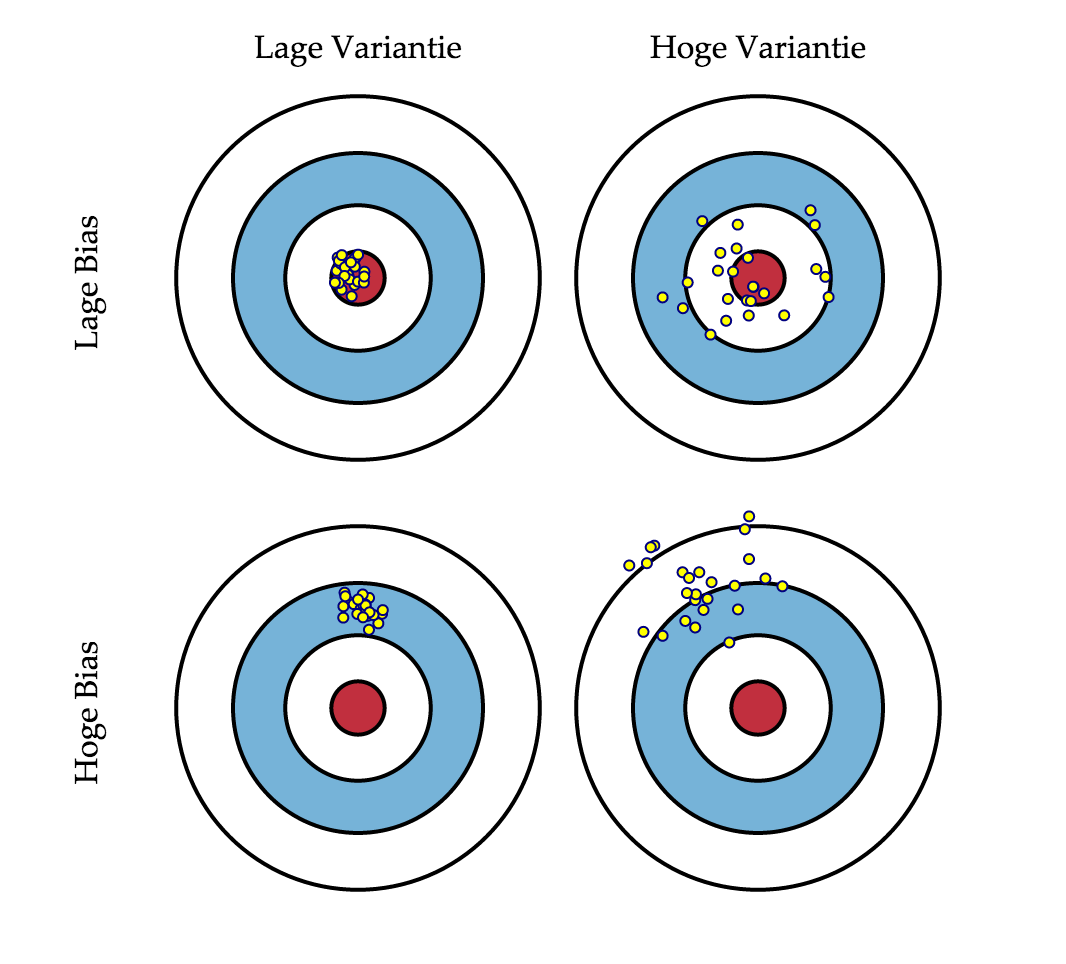
\includegraphics[width=10cm]{bulls-eye}
  \captionof{figure}{Schematische weergave van Bias en Variantie (Gebaseerd op:\url{http://scott.fortmann-roe.com/docs/BiasVariance.html})}
\end{center}
\newline
Concreet kan men zeggen dat wanneer men te maken heeft met bias en variantie, men werkelijk te maken heeft met over- en underfitting. Men spreekt van overfitting wanneer de resultaten op de trainingsset goed zijn, maar voor onbekende sets veel minder.\\
Stel dat we ons model steeds uitbreiden door het te blijven trainen. Als resultaat stijgt de complexiteit van ons model, wat maakt dat het beter voorspellingen kan doen, dus de bias vermindert, maar er gaan meer outliers en afwijkende waarden zijn. Dus de variantie stijgt. Wat dus maakt dat er een trade-off is tussen bias en variantie.\\ 
%
Wiskundig kunnen we dit ook aantonen. Neem $Y$ als de variabele die we willen voorspellen en $X$ als de variabele die de inputwaarden voorstelt. Neem ook aan dat er een relatie bestaat tussen de twee $Y=f(X)$. We willen nu door het algoritme te trainen met de inputwaarden, een hypothese $f_{p}(X)$ maken voor $f(X)$. \\
Neem nu dat we $f(X)$ willen voorspellen door lineaire regressie te gebruiken en de hypothese te beoordelen aan de hand van de squared prediction error. Dit is een metriek om de kwaliteit van de hypothese te bepalen. Hoe hoger de kwaliteit van het model, hoe lager de squared prediction error van het model. Als we nu de formule van squared prediction error er bij nemen:

\[ Err(X)=E[(Y - f_{p}(X))^2] \]
%
met $E$ de verwachtingswaarde.\\
%
Als we deze formule nu herschrijven in functie van bias en variantie componenten (\cite{hastie2009elements}), krijgen we :

\[ Err(X)=(E[f_{p}(X)] - f(X))^2+E[f_{p}(X) - E[f_{p}(X)]]^2 \]
%
Wat neerkomt op 

\[Err(X)= Bias^2 + Variantie \]
%
Hier zien we wederom dat er een keuze moet gemaakt worden tussen de minimalisatie van bias en de minimalisatie van variantie.
Onderstaande afbeelding illustreert nogmaals het verband tussen bias en variantie en hoe deze bijdraagt tot de totale error.
\begin{center}
  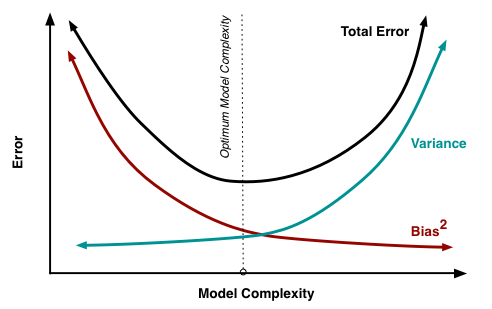
\includegraphics[width=10cm]{biasvariance_tradeoff}
  \captionof{figure}{Bijdrage Bias en Variantie aan totale error (Bron: \url{http://scott.fortmann-roe.com/docs/docs/BiasVariance/biasvariance.png})}
  \label{fig:biasvariance}
\end{center}
\newline
Zoals men kan zien op bovenstaande afbeelding is het optimum voor de complexiteit van het model, de plaats waar de totaal error het laagste is. Als we nog preciser kijken zien we dat dit de plaats is waar de bias evenveel vermindert als de variantie toeneemt. Wiskundig kunnen we dit formuleren als volgt:

\[\frac{dBias}{dComplexiteit} = -\frac{dVariantie}{dComplexiteit} \]
%
In de praktijk is er spijtig genoeg geen analytische methode om dit punt te vinden en moet men samen met de squared predict error functie experimenteren met verschillende levels van complexiteit voor een model en hier het level van complexiteit met de laagste totale error uit selecteren.\\
%
Nu dat we een goed algemeen begrip hebben over bias en variantie, kijken iets dieper in op over- en underfitting.

\subsubsection{Over- en Underfitting}\label{Over- en Underfitting}

Eerder zeiden we al wanneer men spreekt of bias en variantie, men eigelijk bezig is met over- en underfitting. Laten we eerst nog eens kijken wat juist overfitting is. \citet{mitchell1997machine} definieert overfitting als volgt:
\newline
\newline
``\textit{Given a hypothesis space H , a hypothesis h E H is said to overfit the training data if there exists some alternative hypothesis h' E H, such that h has smaller error than h' over the training examples, but h' has a smaller error than h over the entire distribution of instances.}''
\newline
\newline
Wat eigenlijk wil zeggen dat hypothese H te goed werkt op zijn eigen trainingsset, maar als het andere waarden begint te classificeren de prestatie veel minder is. Bij underfitting is het juist omgekeerd. De prestatie is lager op de trainingsset dan op een grote nieuwe dataset. Het te goed presteren van een trainingsset, wil eigelijk zeggen dat het model te precies, te complex is afgesteld. Aan de hand van figuur \ref{fig:biasvariance}, kunnen we afleiden dat dit duidt op een hoge variantie. Gelijkaardig met underfitting, wanneer het getrainde model slecht presteert met zijn eigen trainingsset, wil dit zeggen dat het model te eenvoudig, niet complex genoeg is. Wat duidt op een hoge bias (zie figuur \ref{fig:biasvariance}).
%
Het verband nog eens kort samengevat. Wanneer men spreekt van underfitting, spreekt men van hoge bias. Wanneer men spreekt van overfitting, spreekt men van hoge variantie.
